\documentclass{article}

\usepackage[dutch]{babel}
\usepackage{multicol}
\setlength{\columnsep}{1cm}

\usepackage[a4paper,top=2cm,bottom=2cm,left=2cm,right=2cm,marginparwidth=1.75cm]{geometry}

\usepackage{amsmath}
\usepackage{siunitx}
\usepackage{wrapfig}
\usepackage{float}
\usepackage{graphicx}
\usepackage{subcaption}
\usepackage[colorlinks=true, allcolors=blue]{hyperref}
\usepackage{xcolor}
\usepackage{lipsum}
\usepackage{mathtools}
\usepackage{listings}
\usepackage{xcolor}
\usepackage{pdfpages}




\title{Aandrijftechniek maan casus}

\author{Jelmer Hemstra, 1810225, Flint Wardenaar, 1771881}


\begin{document}
\maketitle

\begin{abstract}
    In dit document wordt de casus van de aandrijftechniek van de rover behandeld. Hierbij wordt gekeken naar de verschillende aandrijftechnieken en de voor- en nadelen van deze technieken.
\end{abstract}


\section{Inleiding}
    In dit document wordt de casus van de aandrijftechniek van de rover behandeld. 


\section{Analyse}
    \subsection{Onderzoeksvragen}
        Hoofdvraag: \newline
        Welke cobinatie van motor en overbrenging, 
        van de familie ``RE25 1187xx'' en ``Planetary Gearhead GP xx xx'' respectievelijk, 
        is het meest geschikt als aandrijving van de ``Euro Moon Rover``?
        \newline \newline
        Deelvragen: 
        \begin{itemize}
            \item Wat is de statische last?
            \item Wat is de dynamische last?
            \item Wat is de meest voorkomende last?
        \end{itemize}

    \subsection{Eisen}
        Uit de opdrachtsbeschrijving zijn de volgende eisen gehaald:
        \begin{enumerate}
            \item De rover moet een helling van $20^{\circ}$ op en af kunnen rijden.
            \item De rover moet kunnen versnellen met $0.7[m/s^2]$ en vertragen met $0.5[m/s^2]$.
            \item De rover moet een topsnelheid hebben van ninstens $2.1[m/s]$.
            \item De motor moet deel uitmaken van de ``RE25 1187xx'' familie en heeft een diameter van 25mm.
            \item De overbrenging moet deel uitmaken van de ``Planetary Gearhead GP xx xx'' familie.
        \end{enumerate}
    
    \subsection{Gegevens}
        Uit de opdracht zijn de volgende gegevens gehaald:
        \begin{itemize}
            \item De massa van de de rover: $m = 6[kg]$
            \item De valversnelling op de maan: $g_m = 1.62[m/s^2]$
            \item De rolweerstandscoëfficiënt: $\mu_r = 0.1$
            \item De straal van de wielen: $r = 0.075[m]$
            \item De massatraagheidvan de wielen: $J = 0.0021[kg \cdot m^2]$
        \end{itemize}
        Ook zijn de eisen genoteerd als gegevens:
        \begin{itemize}
            \item De maximale helling: $\theta_{max} = 20^\circ$
            \item De maximale versnelling: $a_{max} = 0.7[m/s^2]$
            \item De maximale snelheid: $v_{max} = 2.1[m/s]$
        \end{itemize}

\section{Onderzoek}
    Om te bepalen welk type motor het beste is voor de toepassing wordt er vooral gekeken naar de last die de motor moet verdragen.
    De last is opgedeeld in statische en dynamische last. 
    De statische last is de last die de motor moet verdragen als de rover een vaste snelheid heeft.
    De dynamische last is de last die de motor moet verdragen als de rover versnelt of vertraagt.
    \newline
    


    % Beschrijf de aanpak en methoden die gebruikt zijn voor het onderzoek 
    % en de evaluatie van de motoren en transmissiesystemen.
    % Duidelijke formulering van de vraag waarop
    % door middel van analyse/onderzoek een 
    % antwoord wordt gezocht. (max 6 A4’tjes)



    \subsection{Statische last}
        Er zijn twee onderdelen in de statische last, namelijk de zwaartekracht en de rolweerstand. 

        \subsubsection*{Zwaartekracht}
            Met de zwaartekracht wordt de kracht bedoeld die resulteerd uit de kracht die de rover omlaag duwt 
            en de normaalkracht van het oppervlakte. 
            Deze resulterende kracht is ervoor verantwoordelijk dat de rover de helling af ``wil'' rollen.
            Deze is te berekenen met de formule:
            
            \begin{equation}
                F_{z} = m \cdot g \cdot \sin(\theta) 
            \end{equation}

            \begin{itemize}
                \item $F_{z}$ is last die de zwaartekracht veroorzaakt in $[N]$
                \item $m$ is de massa van de rover in $[kg]$
                \item $g$ is de zwaartekracht in $[m/s^2]$
                \item $\theta$ is de hoek van de helling in $[rad]$
            \end{itemize}
        
        \subsubsection*{Rolweerstand}
            De rolweerstand is de kracht die het rollen tegenwerkt en is een gevolg van de frictie tussen de wielen en de grond.
            Deze kracht is te berekenen met de formule:

            \begin{equation}
                F_{rw} =  u_{r} \cdot m \cdot g \cdot \cos(\theta)
            \end{equation}

            \begin{itemize}
                \item $F_{rw}$ is de last die de rolweerstand veroorzaakt in $[N]$
                \item $u_{r}$ is de rolweerstandscoëfficiënt
                \item $g$ is de zwaartekracht in $[m/s^2]$
                \item $\theta$ is de hoek van de helling in $[rad]$
            \end{itemize}

        \subsubsection*{Totaal statische last}
            De totale statische last is dan de som van de zwaartekracht en de rolweerstand:

            \begin{equation}
                F_{stat} = F_{z} + F_{rw}
            \end{equation}

            Om de motor te selecteren moet er gekeken worden naar de koppel. 
            Om de koppel te berekenen per motor moet de volgende formule gebruikt worden:

            \begin{equation}
                T_{stat} = \frac{F_{stat} \cdot r}{4}
            \end{equation}

            Let hierbij op dat de deze last \textbf{per wiel} geldt.



    \subsection{Dynamische last}
        De dynamische last volgt uit twee onderdelen: de massa van de rover en de massatraagheid van de wielen.
        
        \subsubsection*{Massa}
            De last die volgt uit de massa van de rover is te berekenen met de formule:

            \begin{equation}
                T_{m} = m \cdot a \cdot r
            \end{equation}

            \begin{itemize}
                \item $T_{m}$ is het koppel die nodig is om de rover te versnellen $[Nm]$
                \item $m$ is de massa van de rover in $[kg]$
                \item $a$ is de versnelling van de rover in $[m/s^2]$
                \item $r$ is de straal van het wiel in $[m]$
            \end{itemize}
            
        \subsubsection*{massatraagheid}

        De massatraagheid van de wielen is te berekenen met de formule:

        $$T_{inertiawielen} = \frac{I_{wielen} \cdot a}{r_{wiel}}$$
        
        - $T_{inertiawielen}$ is de koppel die het kost om het wiel te versnellen $[Nm]$ \newline
        - $I_{wielen}$ is het traagheidsmoment van de wielen in $[kg \cdot m^2]$ \newline
        - $a$ is de versnelling van de rover in $[m/s^2]$ \newline
        - $r_{wiel}$ is de straal van het wiel in $[m]$ \newline \newline

        De totale dynamische koppel per wiel is dan de som van de massatraagheid van de rover en de massatraagheid van de wielen:
        $$T_{dynamisch per wiel}[Nm] = \frac{T_{inertiarover}[Nm]}{4} + T_{inertiawielen}[Nm] + T_{statischperwiel}[Nm]$$ 


\subsection{Analyse van de motoren}
\subsubsection{gearbox?}

\section{Resultaten}
    Uitkomsten van de analyse, het onderzoek worden gepresenteerd. max 2 A4tjes

    \subsection{last}
    De statische en dynamische lasten zijn berekend voor verschillende hellingen. 
    Uit deze berekeningen zijn de volgende resultaten gekomen: 

        \begin{table}[h]
            \centering
            \begin{tabular}{|c|c|c|c|c|c|}
            \hline
            Helling & $-20 ^\circ$ & $-8.5 ^\circ$ & $0 ^\circ$ & $8.5 ^\circ$ & $20 ^\circ$ \\ \hline
            Statisch [mNm]  & -45.20   & -8.91   & 18.22   & 44.96  & 79.45   \\ \hline
            Dynamisch [mNm]  & 53.13  & 89.43   & 116.57  & 143.31  & 177.81  \\ \hline
            \end{tabular}
            \caption{Helling - Koppel}
            \label{tab}
        \end{table}
        Dit is gedaan met de volgende formules:
        $$T_{statisch} = \frac{r_{wiel}(m \cdot g \cdot sin(\theta) + u_r \cdot m \cdot g \cdot cos(\theta))}{4} = \frac{0.075(9.72 \cdot sin(\theta) +  0.972 \cdot cos(\theta))}{4}$$
        $$T_{dynamisch} = T_{statisch} + \frac{m \cdot a \cdot r_{wiel}}{4} + \frac{I_{wielen} \cdot a}{r_{wiel}} = T_{statisch} + \frac{0.315}{4}+ 0.0196 $$
        Deze formules zijn toegelicht in hoofdstuk 2.1.
        
    \subsection{Motor}
    De motor is gekozen aan de hand van de tabel in 3.1. 
    Ook is er gekeken naar de gearbox daar geldt namenlijk dat hoe minder vertanding de gearbox hoeft te doen hoe efficienter deze is. 
    Hierdoor is er gekozen voor een so traag mogelijke motor binnen de RE25 1187 serie.
    De motor die gekozen is is de RE25 118745. 
    Deze motor heeft een No-load speed van 4790 [rpm], een maximale efficientie van 90 procent en een nominale koppel van 28.7 [mNm].
    De nominale snelheid van de motor is 3710 [rpm].
    

    \subsection{gearhead}
    De gearbox is gekozen aan de hand van de motor. 
    In de datasheet van de motor worden namenlijk een aantal gearboxes aangeraden.
    Een daarvan is degende die wij gekozen hebben, namenlijk de GP 26A 406757. 
    Deze gearbox heeft een vertanding van 5.2:1. dit zorgt voor een Nominale snelheid van 710 [rpm] en een nominale koppel van 150 [mNm]. 
    Dit is meer dan genoeg koppel om met een constante snelheid van 2.1 [m/s] te rijden op een helling van 20 graden.

\section{Advies}
    De


% All other content before appendices should go above this line
% Now, include the PDF files as appendices
% Place this right before the appendix command
\clearpage
\appendix
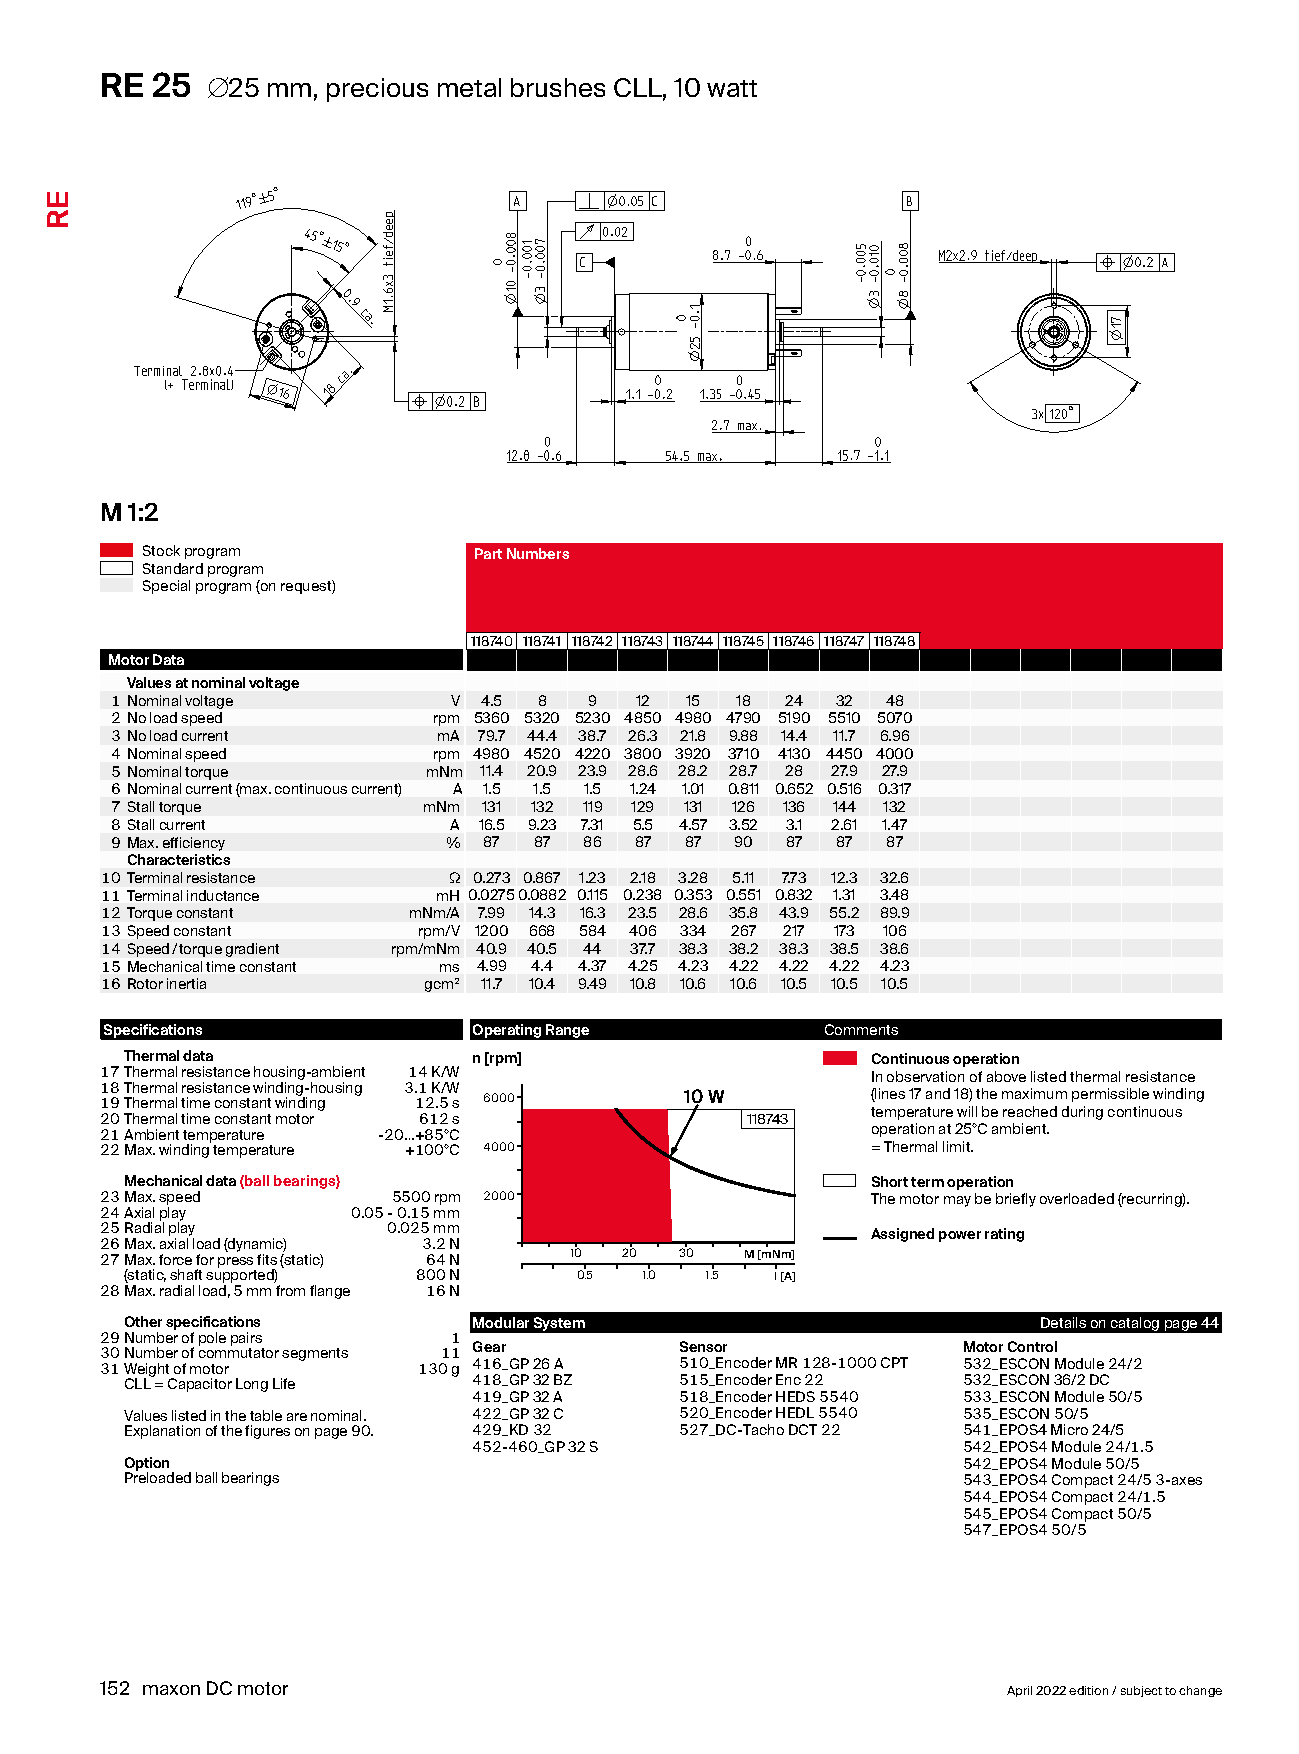
\includepdf[pages=-]{EN-22-152.pdf}
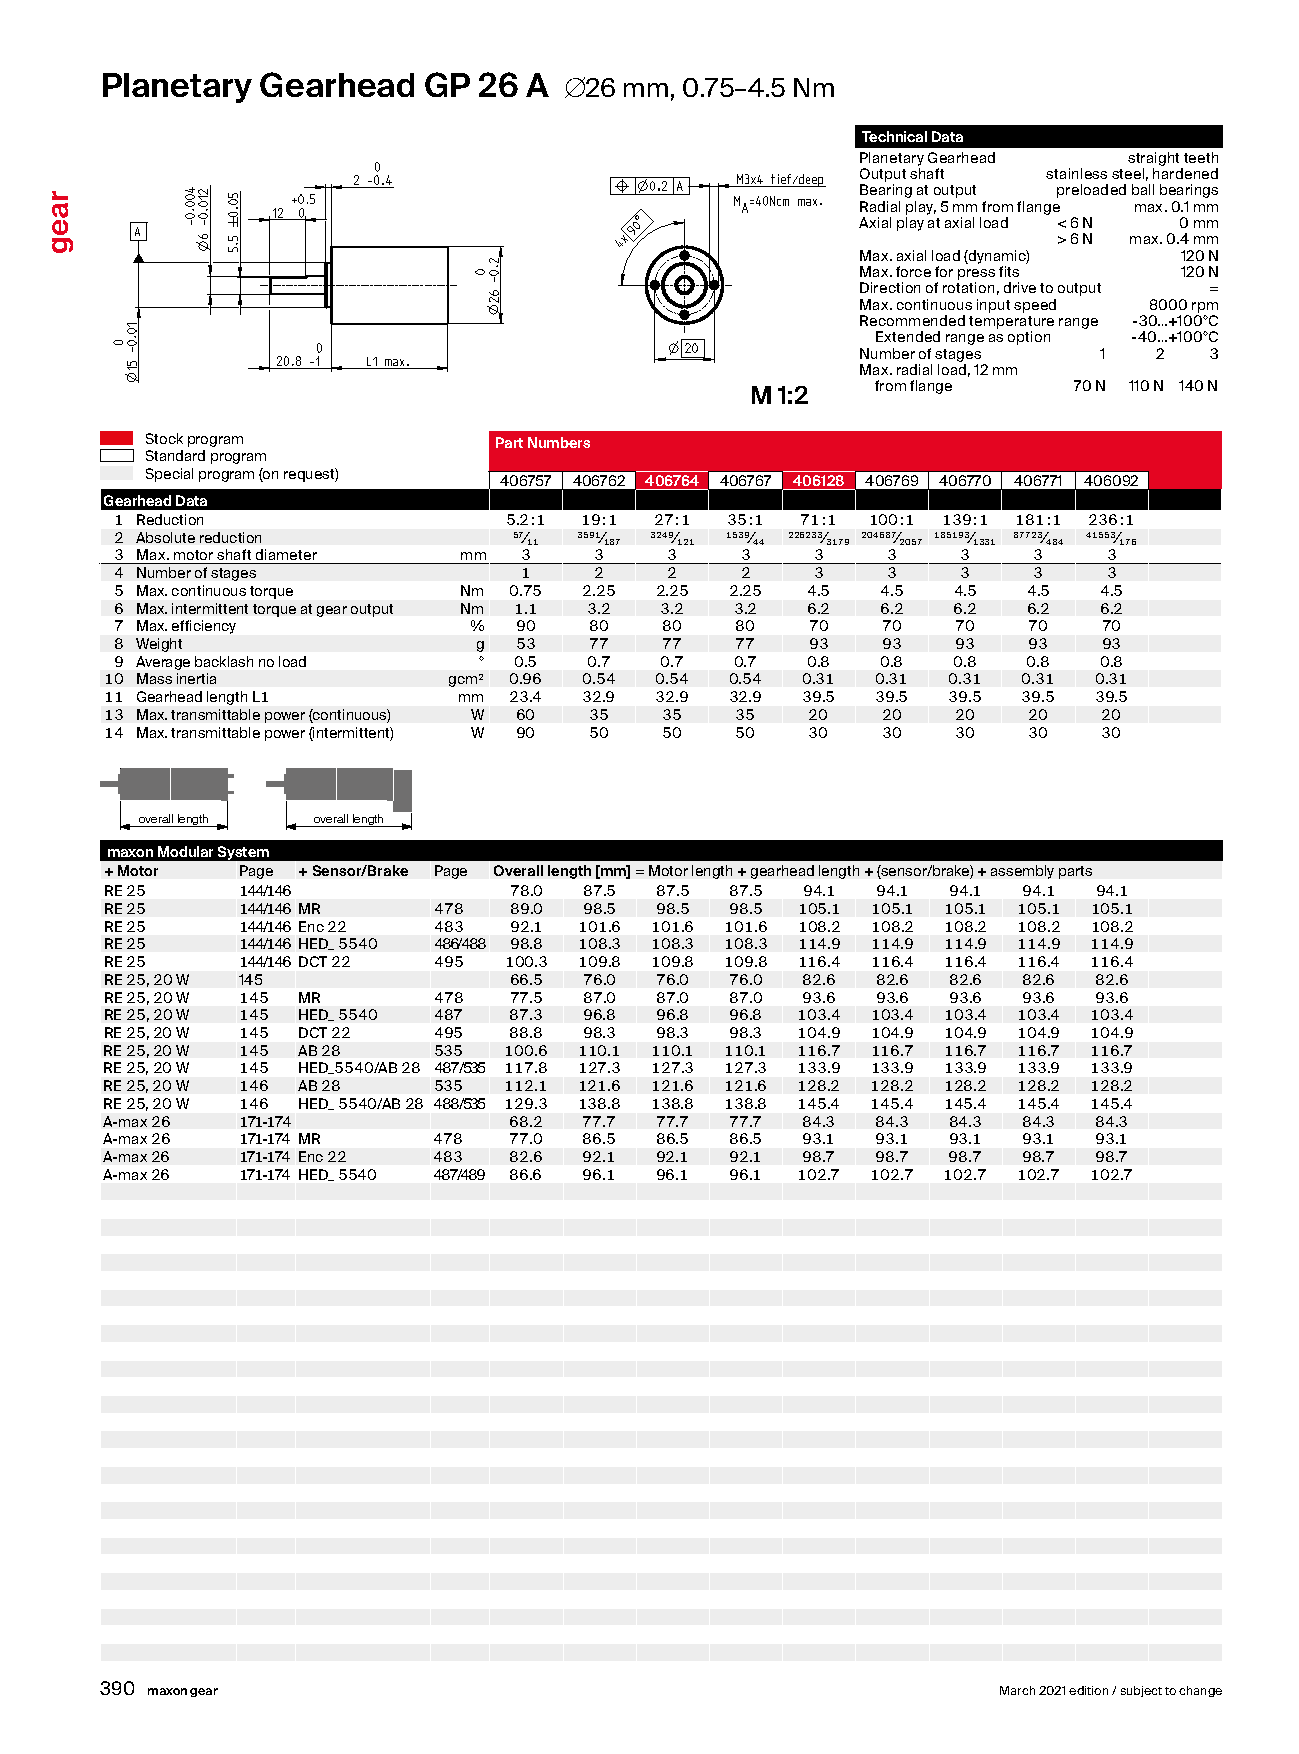
\includepdf[pages=-]{EN-21-390.pdf}

\end{document}